\section{Charectaristics of and Correlations in the Data} % (fold)
\label{sec:Char_Corr}

Before procededing it is a good idea to get a general idea of the correlations between the variables. Figure \ref{fig:Scatter} is a scatter plot showing the dependencies between the \textit{price}, \textit{age}, \textit{km}, and \textit{TIA}. It shows a relavitely strong postive correlation between \textit{price} and \textit{age} and some negative correlation between \textit{age} and \textit{km} as well as negative correlation between \textit{price} and \textit{km}. These relationships are in accord with our existing knowledge of the used car market. \textit{TIA} seems to explain the other variables in this model poorly.

\begin{figure}[H]
  \begin{center}
    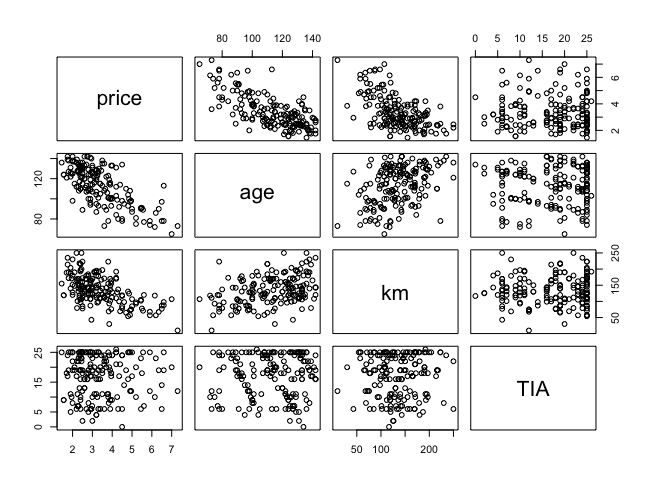
\includegraphics[scale=0.7]{./img/Scatter.png}
    \end{center}
  \caption{Scatter plot of the variables \textit{price}, \textit{age}, \textit{km}, and \textit{TIA}.}
  \label{fig:Scatter}
\end{figure}

\noindent
In addition to this we can use boxplots to analyze whether the presence of ABS technology or a sunroof, represented here by the dummy variables \textit{ABS} and \textit{SunRoof}, have an effect on price. Figure \ref{fig:Bxps} displays this analysis for each variable. To the left the boxplots for vehicles with and without ABS show a few perhaps expected characteristics of the dataset. The median price of a car with ABS is significantly higher than their counterparties (compare 3 200 EUR to 2 625 EUR). Also, the variance of the price of cars having an ABS-technology is much lower than for those that without it. Since $50\%$ of all ``ABS'' cars have a price that ranges between 2.6 and 4 with pretty much no ``ABS'' car having a price higher than 6, where as $50\%$ of all ``Non-ABS'' cars have a price that ranges between 2.5 and 4.5 and a maximum of 7. It can be concluded that the price is somewhat correlated to the dummy variable \textit{ABS}, but not very strongly.

\begin{figure}[H]
  \begin{center}
    \includegraphics[scale=0.5]{./img/bxps.png}
    \end{center}
  \caption{Pairs of boxplots of price of vehicles with and without ABS (left) and sunroofs (right).}
  \label{fig:Bxps}
\end{figure}

\noindent
A similar analysis can be done for the presence of a sunroof. The second set of boxplots in Figure \ref{fig:Bxps} show values for vehicles with and without them. The medians are quite similar for ``Non-OpenRoof'' and ``OpenRoof'' cars. The ``box range'' around the median is smaller for cars with sunroofs, but apart from that they are no visible differences. The correlation between price and OpenRoof seems to be rather small; further analysis is needed to confirm this observed relationship.



% section need_name (end)